\documentclass[a4paper]{article}
\usepackage[T1]{fontenc}			% pacchetto per \chapter
\usepackage[italian]{babel}
\usepackage[italian]{isodate}  		% formato delle date in italiano
\usepackage{graphicx}				% gestione delle immagini
\usepackage{amsfonts}
\usepackage{booktabs}				% tabelle di qualità superiore
\usepackage{amsmath}				% pacchetto matematica
\usepackage{enumitem}				% gestione delle liste
\usepackage{pifont}					% pacchetto con elenchi carini
\usepackage[x11names]{xcolor}		% pacchetto colori RGB
% Link ipertestuali per l'indice
\usepackage{xcolor}
\usepackage[linkcolor=black, citecolor=blue, urlcolor=cyan]{hyperref}
\hypersetup{
	colorlinks=true
}

%\usepackage{showframe}				% visualizzazione bordi
%\usepackage{showkeys}				% visualizzazione etichetta

\newcommand{\dquotes}[1]{``#1''}

\begin{document}
	\author{VR443470}
	\title{Basi di dati}
	\date{\printdayoff\today}
	\maketitle

	\newpage
	
	% indice
	\tableofcontents
	
	\newpage
		
	\section{Introduzione}
	
	\subsection{Sistemi informativi, informazioni e dati}
	
	Ogni organizzazione è dotata di un \textbf{\emph{sistema informativo}}, che organizza e gestisce le informazioni necessarie per perseguire gli scopi dell'organizzazione stessa. Per indicare la \textbf{porzione automatizzata del sistema informativo} viene di solito utilizzato il termine \textbf{\emph{sistema informatico}}.
	
	Nei sistemi informatici le informazioni vengono rappresentate per mezzo di \emph{dati}, che hanno bisogno di essere interpretati per fornire informazioni. Esiste una differenza sottile tra dato e informazioni. Solitamente i primi, se presi da soli, non hanno significato, ma, una volta interpretati e correlati opportunamente, essi forniscono informazioni, che consentono di arricchire la conoscenza:

	\begin{description}
		\item[\textbf{Informazione}:] notizia, dato o elemento che consente di avere conoscenza più o meno esatta di fatti, situazioni, modi di essere;
		\item[\textbf{Dato}:] ciò che è immediatamente presente alla conoscenza, prima di ogni elaborazione. In informatica, sono elementi di informazione costituiti da simboli che devono essere elaborati.
	\end{description}
	
	\noindent
	\textcolor{Red3}{\textbf{[ESAME] Definizione base di dati}}: Una \textbf{\emph{base di dati}} è una collezione di dati, utilizzati per rappresentare con tecnologia informatica le informazioni di interesse per un sistema informativo.
	
	\newpage
	
	
	
	\subsection{Basi di dati e sistemi di gestione di basi di dati}
	
	Inizialmente, venne adottato un \dquotes{\underline{approccio convenzionale}} alla gestione dei dati. Esso \textbf{sfruttava} la presenza di archivi o \textbf{file per memorizzare} e \textbf{per ricercare dati}. Tuttavia, i metodi di accesso e condivisione erano semplici e banali.\newline
	Infatti, erano presenti numerosi \textbf{problemi}:
	
	\begin{itemize}
		\item[\ding{56}] \textbf{Accesso sequenziale}: la scarsa efficienza nell'accesso ai dati su file rendeva lento l'accesso a tali informazioni;
		\item[\ding{56}] \textbf{Ridondanza}: i dati di interesse per più programmi sono replicati tante volte quanti sono i programmi che li utilizzano, con evidente ridondanza e possibilità di incoerenza;
		\item[\ding{56}] \textbf{Inconsistenza}: una diretta conseguenza della ridondanza. Con la presenza di più copie di un determinato dato, l'eventuale cambiamento di uno solo potrebbe portare a questo effetto;
		\item[\ding{56}] \textbf{Progettazione duplicata}: per ogni programma viene replicata la progettazione.
	\end{itemize}
	
	\noindent
	La \textbf{soluzione} è arrivata negli anni '80 con l'avvento delle \textbf{basi di dati}. Quest'ultime gestiscono in modo integrato e flessibile le informazioni di interesse per diversi soggetti.\newline
	\newline \noindent	
	\textcolor{Red3}{\textbf{[ESAME] Definizione DBMS}}: Un \textbf{\emph{sistema di gestione di basi di dati}} (in inglese \emph{Data Base Management System}, \textbf{DBMS}) è un sistema software in grado di gestire collezioni di dati che siano:
	
	\begin{itemize}
		\item[\ding{52}] \textbf{Grandi};
		\item[\ding{52}] \textbf{Condivise};
		\item[\ding{52}] \textbf{Persistenti}.
	\end{itemize}
	
	\noindent
	\underline{assicurando} allo stesso tempo:
	
	\begin{itemize}
		\item[\ding{72}] \textbf{Affidabilità};
		\item[\ding{72}] \textbf{Privatezza};
		\item[\ding{72}] \textbf{Accesso efficiente}.
	\end{itemize}

	Il \textbf{vantaggio} di utilizzare un DBMS è stato evidenziato nella definizione. Quindi:
	
	\begin{itemize}
		\item[\ding{51}] \textbf{Maggiore astrazione} poiché le sue funzioni \underline{estendono il \emph{file system}}, fornendo la possibilità di accesso condiviso agli stessi dati da parte di più utenti e applicazioni;
		\item[\ding{51}] \textbf{Maggiore efficacia} poiché le operazioni di accesso ai dati si basano su un linguaggio di interrogazione.
	\end{itemize}
	
	
	
	
	\subsection{Linguaggi per basi di dati}
	Su un DBMS è possibile specificare operazioni di vario tipo, ma principalmente si distinguono in due categorie:

	\begin{itemize}
		\item \textbf{Linguaggi di definizione dei dati} (\emph{Data Definition Language}, abbreviato con \textbf{DDL}) utilizzati per \underline{definire} gli \underline{schemi logici}, \underline{esterni} e \underline{fisici} e le \underline{autorizzazioni per l'accesso};
		\item \textbf{Linguaggi di manipolazione dei dati} (\emph{Data Manipulation Language}, abbreviato con \textbf{DML}) \underline{utilizzati} per l'\underline{interrogazione} e l'\underline{aggiornamento} delle \underline{istanze} di basi di dati:
		\begin{itemize}
			\item \emph{Linguaggio di interrogazione}, estrae informazioni da una base di dati (SQL, algebra relazionale);
			\item \emph{Linguaggio di manipolazione}, popola la base di dati, modifica il suo contenuto con aggiunte, cancellazioni e variazioni sui dati (SQL).
		\end{itemize}
	\end{itemize}
	
	\newpage
	
	
	
	
	\subsection{Modelli dei dati}
	\textcolor{Red3}{\textbf{Definizione modello dei dati}}: Un \textbf{\emph{modello dei dati}} è un insieme di concetti utilizzati per organizzare i dati di interesse e descriverne la struttura in modo che essa risulti comprensibile ad un elaboratore.
	
	Ogni modello dei dati fornisce \textbf{meccanismi di strutturazione}, analoghi ai \textbf{\emph{costruttori}} di tipo dei linguaggi di programmazione (es: Java), che permettono di definire nuovi tipi sulla base di tipi predefiniti (elementari) e costruttori di tipo. Quindi, i \emph{costruttori} consentono di:
	
	\begin{itemize}
		\item[\ding{43}] \textbf{\emph{Definire}} le \textbf{strutture dati che conterranno le informazioni} della base di dati;
		\item[\ding{43}] \textbf{\emph{Specificare}} le \textbf{proprietà che dovranno soddisfare le istanze} di informazione che saranno contenuto nelle strutture dati.
	\end{itemize}

	\noindent \newline
	\textcolor{Red3}{\textbf{Definizione schemi e istanze}}: È molto importante distinguere gli \textbf{schemi} e le \textbf{istanze} dal concetto di modello dei dati:
	
	\begin{itemize}
		\item \textbf{\emph{Schema}}: parte \underline{invariante nel tempo}, è costituita dalle caratteristiche dei dati. In altre parole, è la descrizione della struttura e delle proprietà di una specifica base di dati fatta utilizzando i costrutti del modello dei dati;
		\item \textbf{\emph{Istanza} o \emph{stato}}: parte \underline{variabile nel tempo}, è costituita dai valori effettivi. Quest'ultimi, in un certo istante, popolano le strutture dati della base di dati.
	\end{itemize}

	\begin{figure}[!htp]
		\centering
		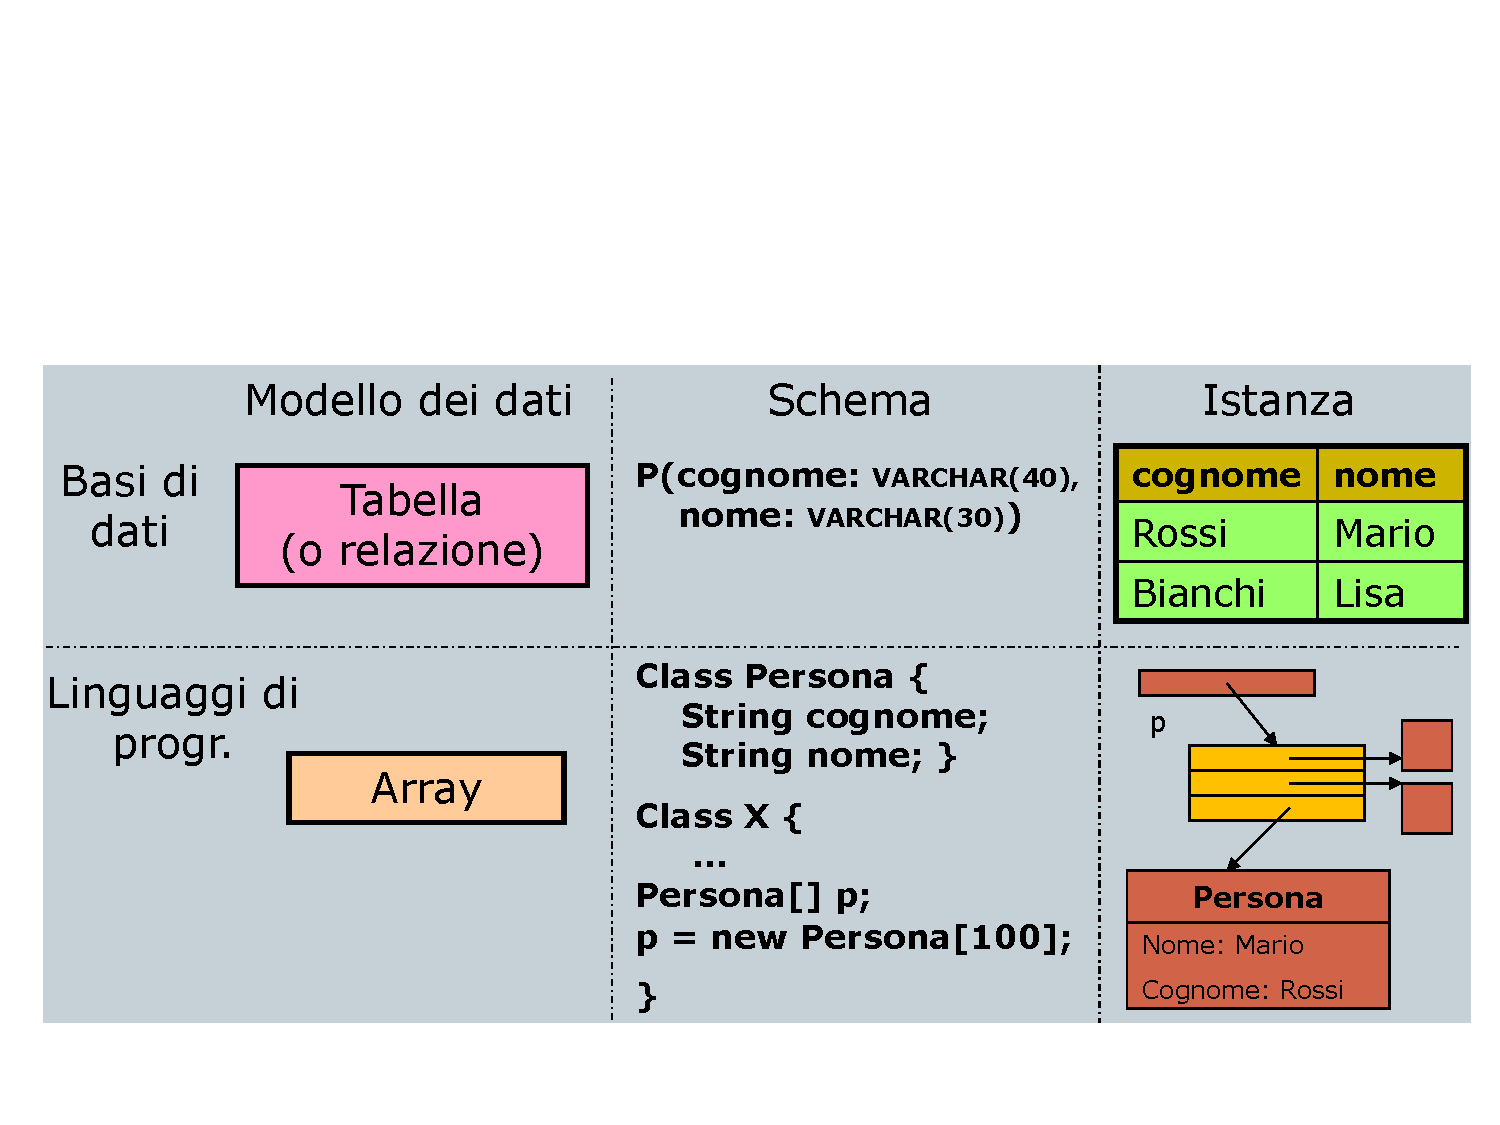
\includegraphics[width=0.9\textwidth]{img/diff_modello-schemi-istanze.pdf}
		\caption{Esempio di modello di dati, schema e istanza.}
	\end{figure}

	\newpage
	
	
	
	
	\subsection{Astrazione (architettura) dei DBMS}\label{Astrazione (architettura) dei DBMS}
	
	Esiste un'architettura standardizzata per i DMBS, la quale si caratterizza su tre livelli: \textbf{esterno}, \textbf{logico} e \textbf{interno}:
	
	\begin{itemize}
		\item[\ding{80}] \textbf{\emph{Schema logico.}} È la rappresentazione della \textbf{struttura} e delle \textbf{proprietà} della \textbf{base di dati} definita \underline{attraverso i costrutti} del modello dei dati del DBMS. In altre parole, descrive l'intera base di dati per mezzo del modello logico adottato dal DBMS (quindi relazione o ad oggetti).
		
		\item[\ding{72}] \textbf{\emph{Schema interno.}} È la rappresentazione della base di dati per mezzo delle \textbf{strutture fisiche di memorizzazione} (e.g. file sequenziale, file hash, ecc.).
		
		\item[\ding{73}] \textbf{\emph{Schema esterno.}}\label{schema esterno} Descrive una \textbf{porzione dello schema logico} di interesse per uno \textbf{specifico} utente o applicazione. \underline{Possono esistere più schemi} esterni che consentono di avere \underline{punti di vista differenti} senza cambiare la logica di base.
	\end{itemize}

	\begin{figure}[!htp]
		\centering
		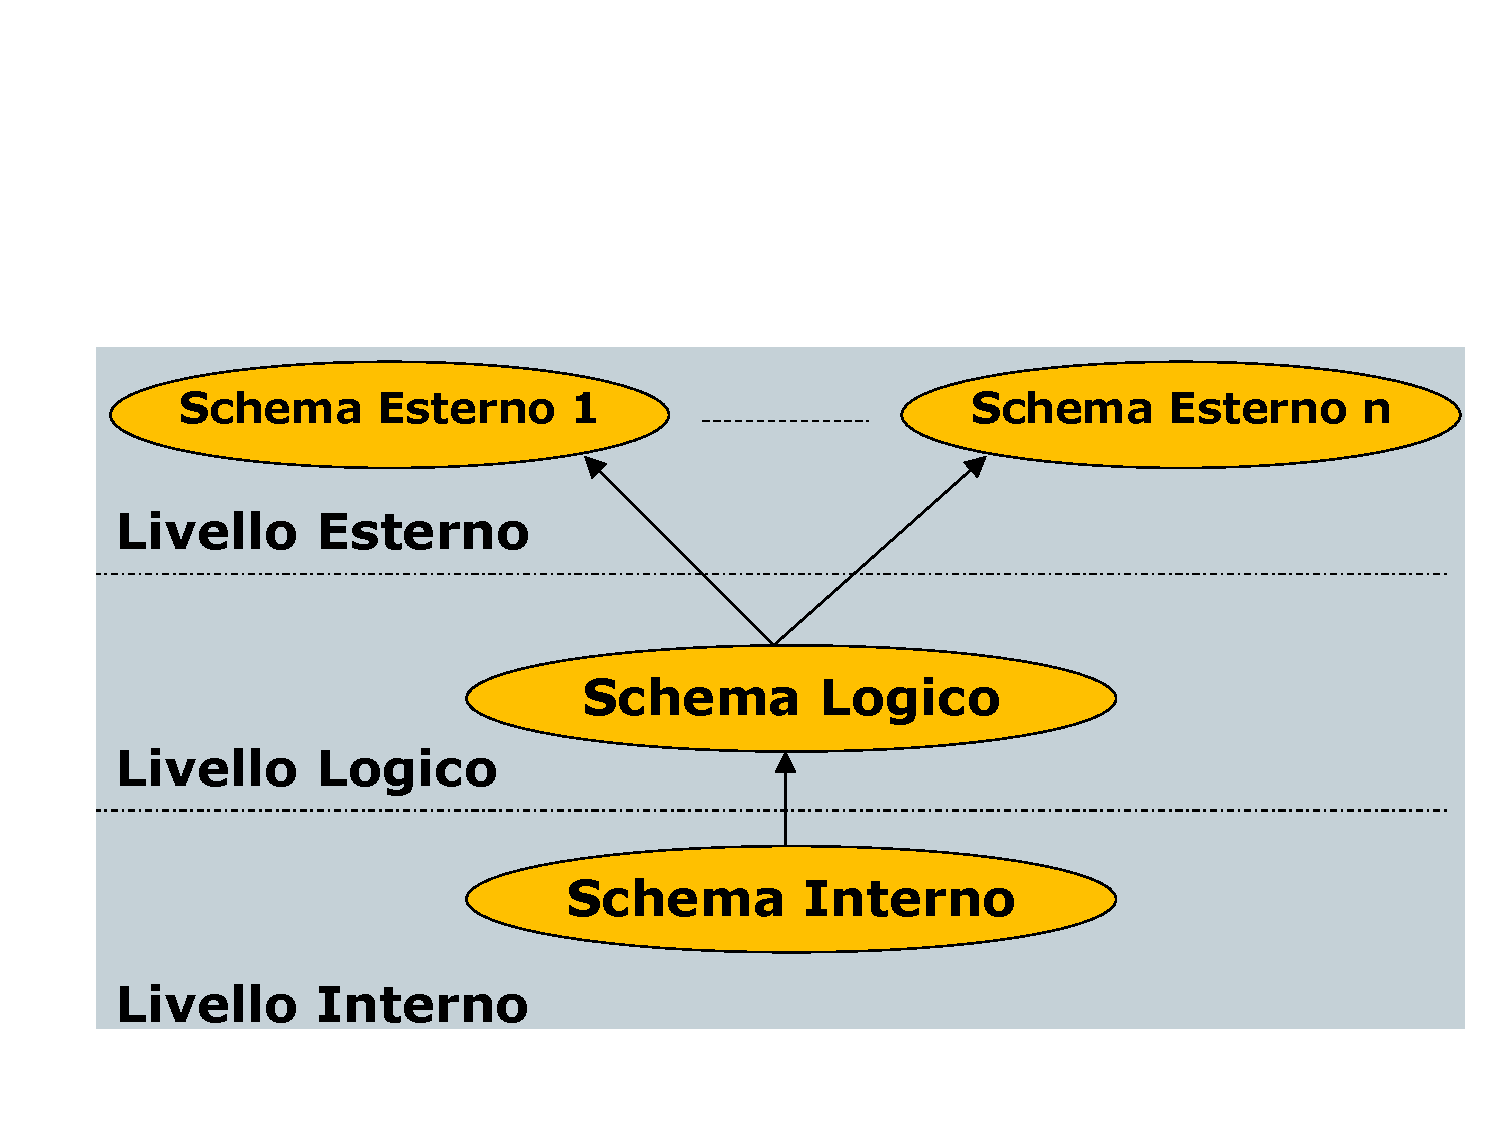
\includegraphics[width=0.8\textwidth]{img/arch_DBMS.pdf}
		\caption{Architettura generale di un DBMS.}
	\end{figure}

	\newpage
	
	
	
	
	\subsection{Indipendenza dei dati}
	
	L'architettura a livelli definita nel paragrafo \ref{Astrazione (architettura) dei DBMS} garantisce l' \textcolor{Red3}{\textbf{indipendenza dei dati}}, la \textbf{proprietà più importante} dei DBMS. L'\textbf{obbiettivo} è quello di poter fornire all'utente una basi di dati in grado di interagire con un \underline{elevato livello di astrazione}. Esistono due tipi di indipendenza:
	
	\begin{itemize}
		\item[\ding{42}] \textbf{\emph{Indipendenza \underline{fisica}.}} Lo schema logico della basi di dati è \underline{completamente} indipendente dallo schema interno. Quindi, l'interazione con il DBMS può essere effettuato in modo indipendente dalla struttura fisica dei dati.\newline
		\textcolor{Green4}{\textbf{Vantaggio:}} le modifiche \textbf{\underline{non}} influiscono sullo schema logico, cioè sulle applicazioni che lo utilizzano.
		
		\item[\ding{42}] \textbf{\emph{Indipendenza \underline{logica}.}} Gli \underline{schemi esterni} (definizione nel paragrafo:~\ref{schema esterno}) della base di dati sono \textbf{\underline{indipendenti}} dallo \underline{schema logico}. Quindi, è possibile interagire con il livello esterno in modo indipendente dal livello logico.\newline
		\textcolor{Green4}{\textbf{Vantaggio:}}
		\begin{enumerate}[label=\Roman*]
			\item \textbf{Aggiunta/Modifica} di uno schema \underline{esterno} in base alle esigenze di un nuovo utente, senza modificare lo schema logico;
			
			\item \textbf{Modifica} di uno schema logico mantenendo inalterate le strutture esterne.
		\end{enumerate}
	\end{itemize}

	\newpage
	
	


	\section{Metodologie e modelli per il progetto}
	
	\subsection{Ciclo di vita dei sistemi informativi}
	
	La progettazione di una base di dati costituisce solo una delle componenti del processo di sviluppo di un sistema informativo complesso e va quindi inquadrata in un contesto più ampio quello del \textbf{ciclo di vita} dei sistemi informativi:
	
	\begin{itemize}
		\item[\ding{42}] \textbf{\emph{Studio di fattibilità.}} Definisce i \underline{costi} delle varie alternative possibili e stabilisce le \underline{priorità di realizzazione} delle varie componenti del sistema.
		
		\item[\ding{42}] \textbf{\emph{Raccolta e analisi dei requisiti.}} Individua le proprietà e le funzionalità che il sistema informativo deve avere producendo una descrizione completa, ma generalmente informale.
		
		\item[\ding{42}] \textbf{\emph{Progettazione.}} Si divide in due fasi:
		\begin{itemize}
			\item \textbf{Progettazione dei dati.} Individua la struttura e l'organizzazione che i dati devono avere.
			
			\item \textbf{Progettazione delle applicazioni.} Definizione delle caratteristiche dei programmi applicativi.
		\end{itemize}
		
		\item[\ding{42}] \textbf{\emph{Implementazione (su un DBMS).}} È la realizzazione del sistema informativo secondo la struttura e le caratteristiche fornite durante la fase di progettazione. In questa fase \underline{viene costruita e popola la base di dati}.
		
		\item[\ding{42}] \textbf{\emph{Validazione e collaudo.}} Verifica il corretto funzionamento e la qualità del sistema informativo.
		
		\item[\ding{42}] \textbf{\emph{Funzionamento.}} Il sistema informativo diventa operativo ed esegue i compiti per i quali è stato progettato.
	\end{itemize}

	\noindent
	Spesso il processo \textbf{non} è strettamente sequenziale. Infatti, come si vede dalla seguente figura, durante l'esecuzione di una delle attività sopraelencate, è necessario rivedere decisioni prese nell'attività precedente.
	
	\begin{figure}[!htp]
		\centering
		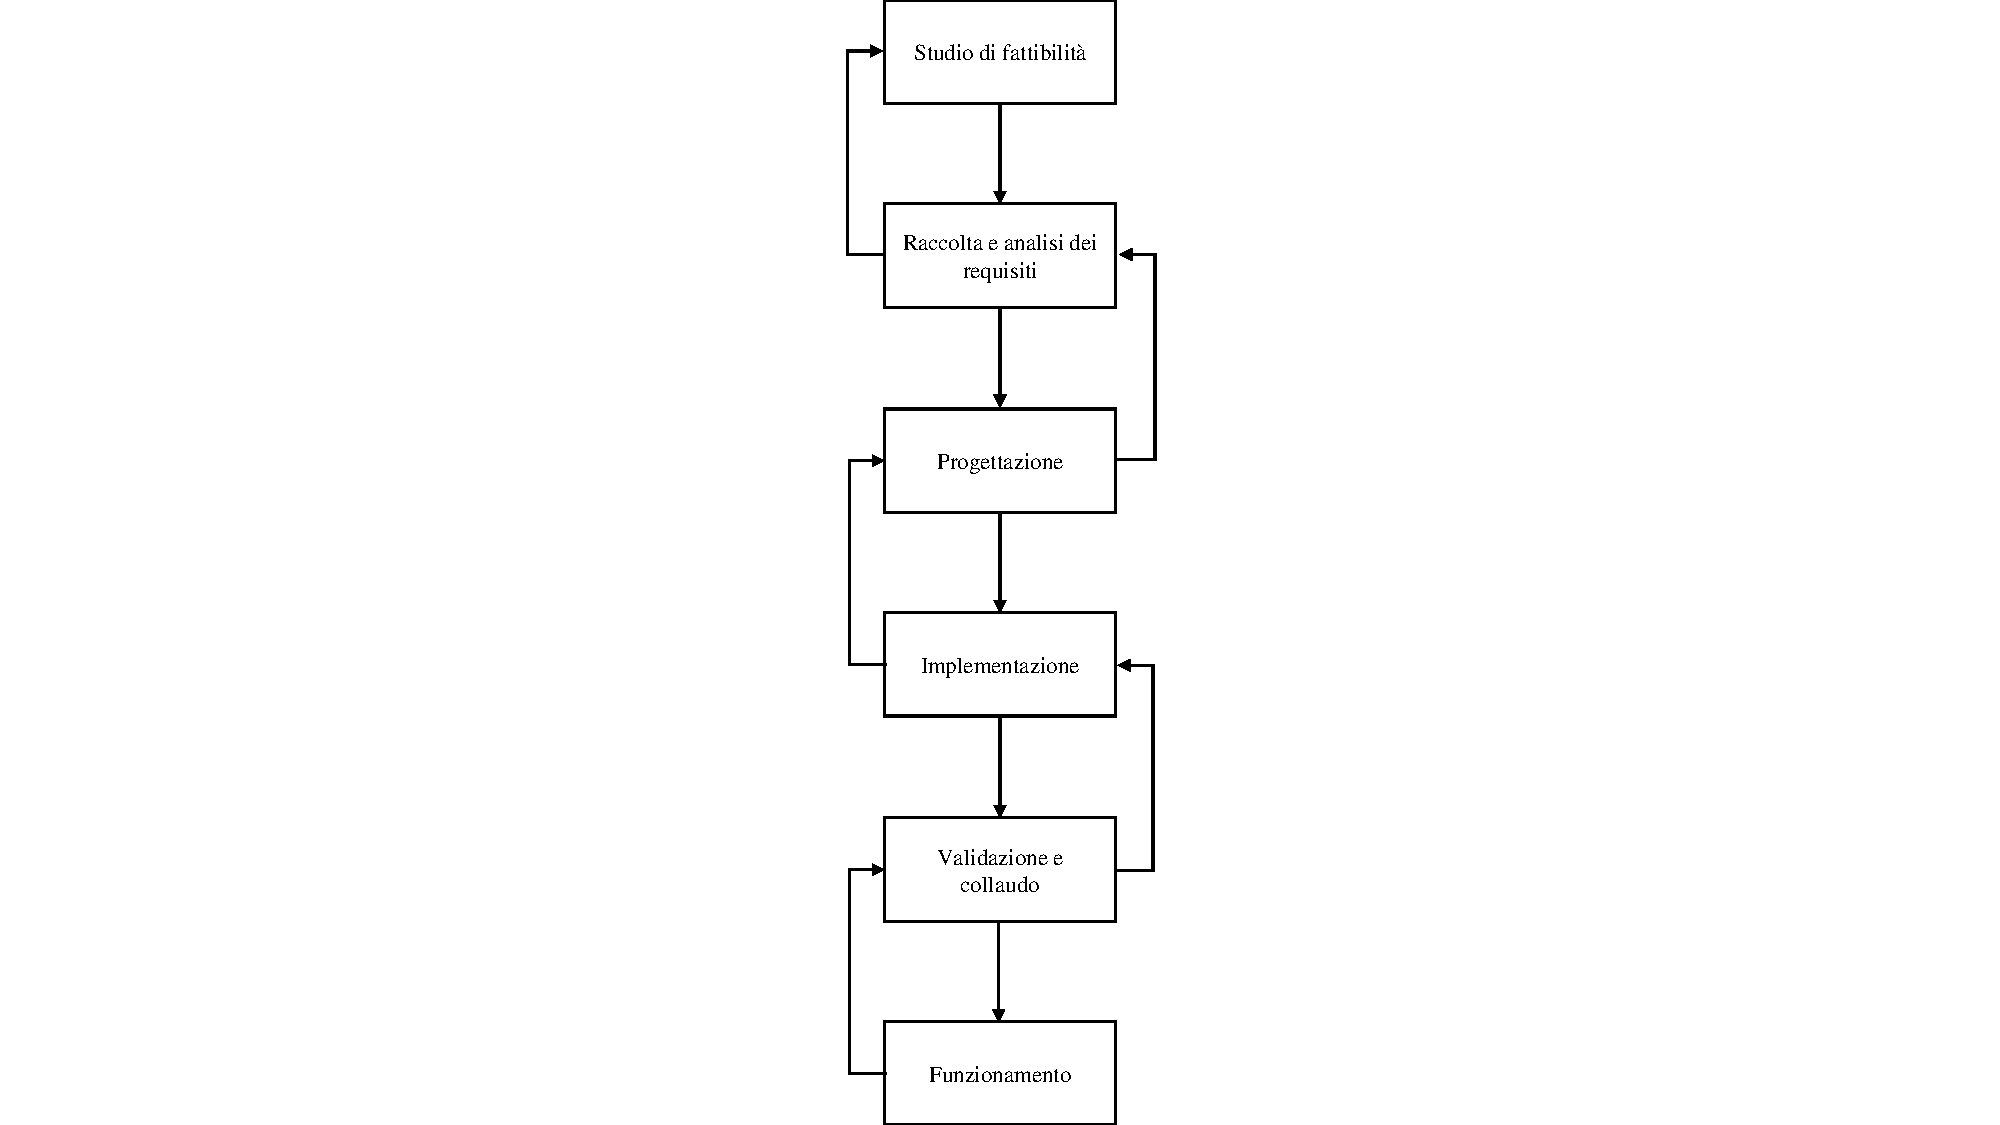
\includegraphics[width=0.4\textwidth]{img/ciclo_di_vita_sis_inf.pdf}
		\caption{Ciclo di vita di un sistema informativo.}
	\end{figure}

	\newpage
	
	
	
	
	\subsection{Metodologie di progettazione e basi di dati}
	
	Una \textbf{metodologia di progettazione} consiste in:
	
	\begin{itemize}
		\item[\ding{51}] \textbf{Decomposizione} dell'intera attività di progetto in passi successivi indipendenti tra loro.
		
		\item[\ding{51}] \textbf{Strategie} da seguire nei vari passi e \textbf{criteri} nel caso di alternative.
		
		\item[\ding{51}] \textbf{Modelli di riferimento} per descrivere i dati in ingresso e uscita delle varie fasi.
	\end{itemize}

	\noindent
	Le \textbf{proprietà} che una metodologia deve garantire sono:
	
	\begin{itemize}
		\item[\ding{72}] \textbf{\emph{Generalità}} rispetto alle applicazioni e ai sistemi in gioco;
		
		\item[\ding{72}] \textbf{\emph{Qualità del prodotto}} in termini di correttezza, completezza ed efficienza rispetto alle risorse impiegate;
		
		\item[\ding{72}] \textbf{\emph{Facilità d'uso}} delle strategie e dei modelli di riferimento.
	\end{itemize}

	%\newpage

	Negli anni si è \emph{consolidata una metodologia} di progetto che ha dato prova di soddisfare pienamente le proprietà descritte. Si basa sull'idea di separare le decisioni relative a \dquotes{cosa} rappresentare in una base di dati (prima fase), da quelle relative a \dquotes{come} farlo (seconda e terza fase):
	
	\begin{itemize}
		\item[\ding{42}] \textbf{Progettazione concettuale.}\newline
		\textcolor{Red3}{\textbf{Obbiettivo:}} rappresentare le specifiche informali della realtà di interesse in termini di una descrizione formale e completa. La \textbf{\underline{rappresentazione}} \textbf{\underline{deve essere indipendente}} dai criteri di rappresentazione utilizzati nei sistemi di gestione di basi di dati.\newline
		\textcolor{Green4}{\textbf{Prodotto di questa fase:}} \underline{schema concettuale}. È un documento formale che rappresenta il contenuto della base di dati in modo indipendente dall'implementazione (DBMS).\newline
		\textcolor{Blue3}{\textbf{Applicazione:}} cercare di rappresentare il \textbf{contenuto informativo} della base di dati, senza preoccuparsi né della modalità con le quali queste informazioni verranno codificate in un sistema reale, né dell'efficienza dei programmi che faranno uso di queste informazioni.\label{progettazione concettuale}
		
		\item[\ding{42}] \textbf{Progettazione logica.}\newline
		\textcolor{Red3}{\textbf{Obbiettivo:}} traduzione dello schema concettuale prodotto nella fase precedente, in termini del modello di rappresentazione dei dati adottato dal sistema di gestione di base di dati a disposizione.\newline
		\textcolor{Green4}{\textbf{Prodotto di questa fase:}} \underline{schema logico}.\newline
		\textcolor{Blue3}{\textbf{Applicazione:}} durante la traduzione, le scelte progettuali si \underline{devono} basare anche su criteri di ottimizzazione delle operazioni da effettuare sui dati.\label{progettazione logica}
		
		\item[\ding{42}] \textbf{Progettazione fisica.}\newline
		\textcolor{Red3}{\textbf{Obbiettivo:}} lo schema logico viene completato con la specifica dei parametri fisici di memorizzazione dei dati.\newline
		\textcolor{Green4}{\textbf{Prodotto di questa fase:}} \underline{schema fisico}.\newline\label{progettazione fisica}
	\end{itemize}

	\newpage
	
	
	
	
	\subsection{Il modello Entità-Relazione (E-R)}
	
	Il \textcolor{Red3}{\textbf{\emph{modello Entità-Relazione}}} è un modello \textbf{concettuale} di dati, quindi utilizzato nella \textbf{progettazione concettuale}, e fornisce una serie di strutture, chiamati \textbf{\emph{costrutti}}, atte a descrivere la realtà di interesse in una maniera facile da comprendere e che prescinde dai criteri di organizzazione dei dati nei calcolatori.
	
	I \underline{costrutti vengono utilizzati} per \textbf{definire schemi} che \textbf{descrivono l'organizzazione e la struttura delle occorrenze} (o \textbf{istanze}) \textbf{dei dati}, ovvero, dei valori assunti dai dati al variare del tempo.
	
	\noindent
	Si possono \underline{riassumere le caratteristiche} del modello Entità-Relazione:
	
	\begin{itemize}
		\item[\ding{42}] \textcolor{SpringGreen4}{\textbf{\emph{Modello concettuale}.}} Utilizzato durante la progettazione concettuale (definizione al paragrafo~\ref{progettazione concettuale}) di una base di dati.
		
		\item[\ding{42}] \textcolor{SpringGreen4}{\textbf{\emph{Strumenti formali}.}} Vengono messi a disposizione diversi strumenti per definire la \textbf{struttura} e le \textbf{proprietà} di una base di dati (\emph{esempio i costrutti}).
		
		\item[\ding{42}] \textcolor{SpringGreen4}{\textbf{\emph{Indipendente dalla tecnologia}.}} Essendo un modello astratto, l'obbiettivo è quello di definire la struttura e le proprietà della base di dati (\underline{non di implementarla!}).
		
		\item[\ding{42}] \textcolor{SpringGreen4}{\textbf{\emph{Formale}.}} È facile da utilizzare nonostante non ammetta ambiguità.
		
		\item[\ding{42}] \textcolor{SpringGreen4}{\textbf{\emph{Grafico}.}} La sintassi è prettamente grafica e questo aumenta anche la leggibilità.
	\end{itemize}

	\newpage
	
	
	
	
	\subsection{I costrutti principali del modello}
	
	Si analizzano i principali costrutti di questo modello: entità (pagina~\pageref{entità}), relazioni(pagina~\pageref{relazioni}) e attributi (pagina~\pageref{attributi}).
	
	\subsubsection{Entità}\label{entità}
	\textcolor{Red3}{\textbf{Definizione.}} Rappresentano \textbf{classi di oggetti} (per esempio, fatti, cose, persone) \textbf{che hanno proprietà comuni ed esistenza \dquotes{autonoma} ai fini dell'applicazione di interesse}. Per esempio, \dquotes{città, dipartimento, impiegato, acquisto e vendita} sono entità di un'applicazione aziendale. Inoltre, \textbf{ogni entità ha un nome identificativo}, il quale deve essere \textbf{univoco}. In sintesi:
	
	\begin{itemize}
		\item Hanno \textbf{proprietà comuni};
		\item Hanno \textbf{esistenza autonoma};
		\item Hanno \textbf{identificazione univoca}.
	\end{itemize}

	\noindent
	\textcolor{Green4}{\textbf{Sintassi grafica.}}
	
	\begin{figure}[!htp]
		\centering
		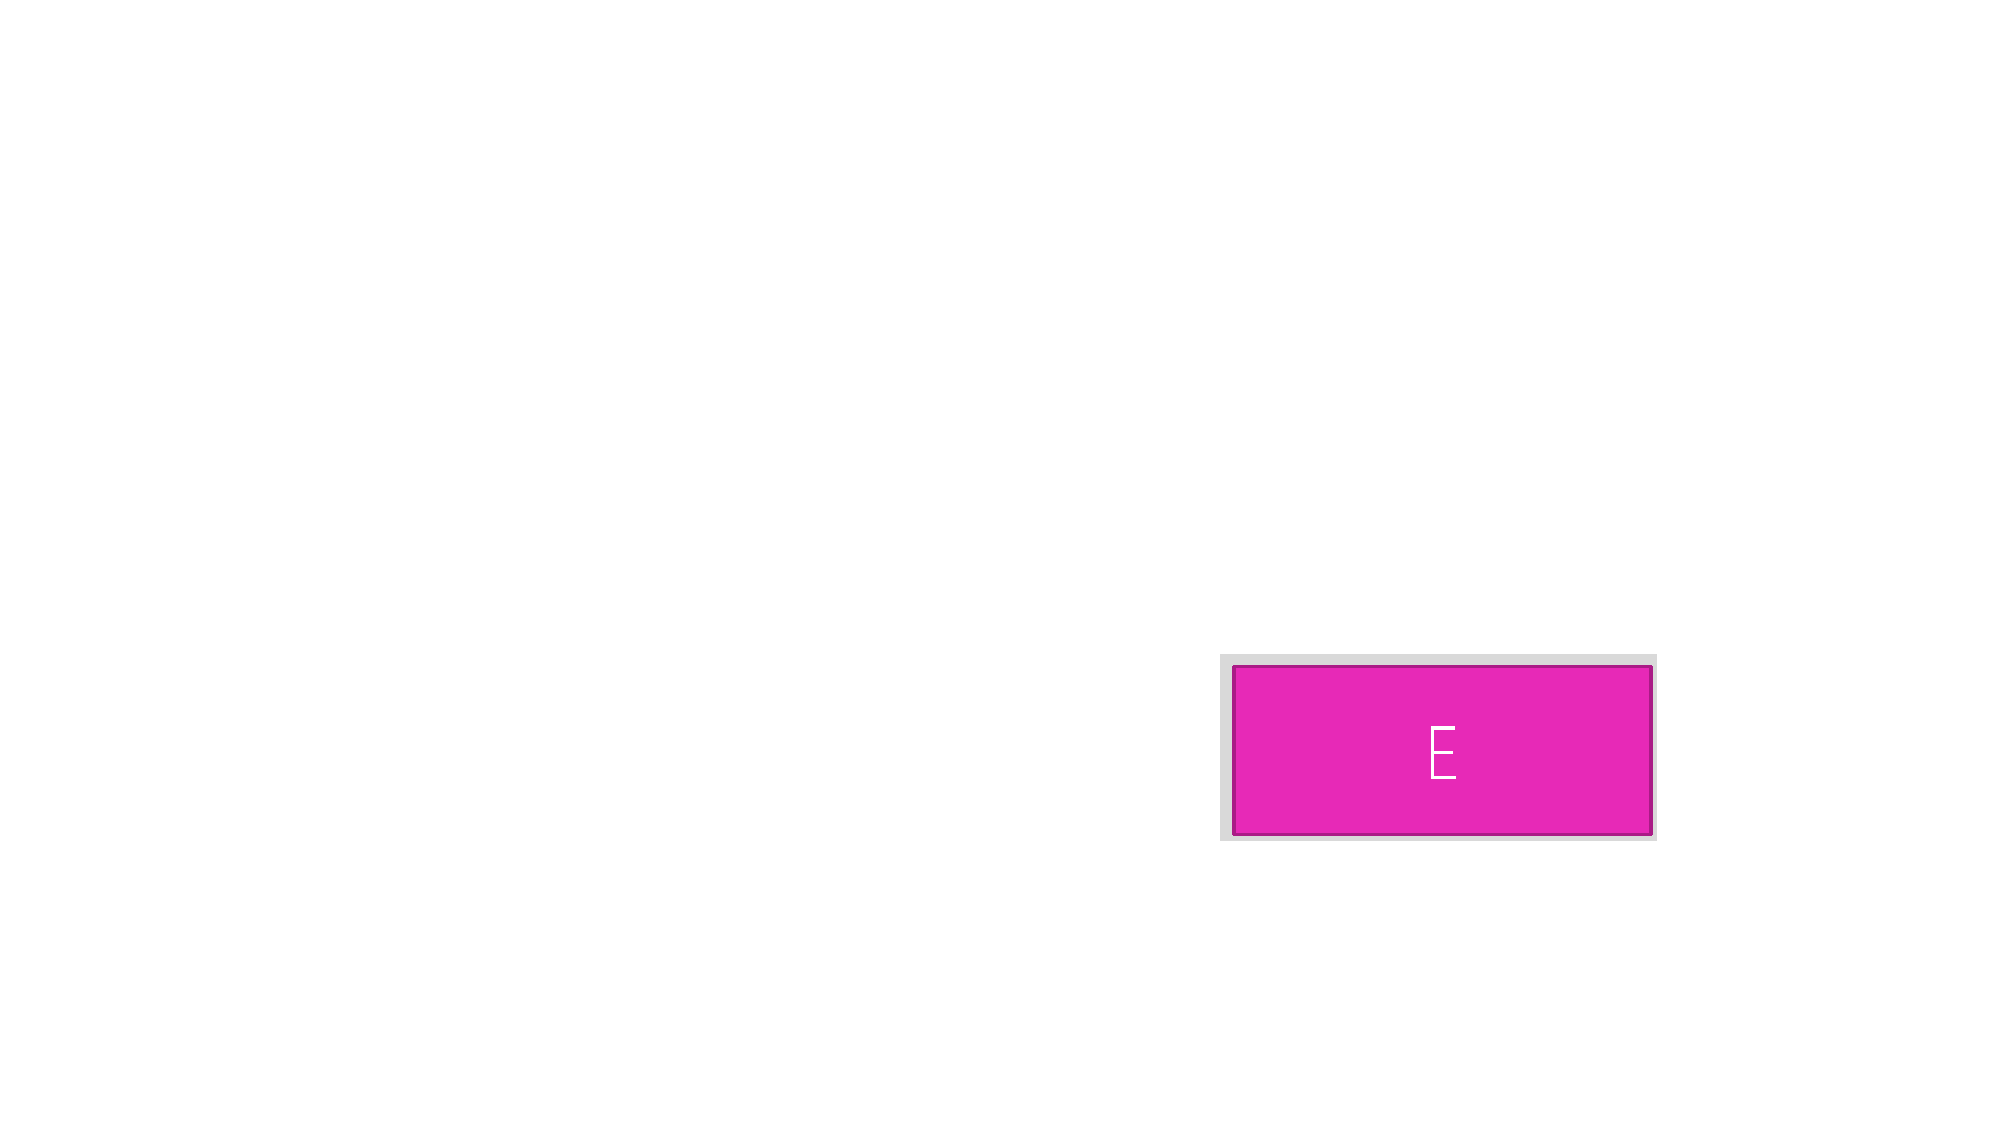
\includegraphics[width=0.5\textwidth]{img/entita_def.pdf}
		\caption{Sintassi grafica dell'entità.}
	\end{figure}

	\noindent
	\textcolor{blue}{\textbf{Istanza (o occorrenza).}} Un'\textbf{istanza} (o occorrenza) di un'entità è un \textbf{oggetto della classe che l'entità rappresenta}. Le città di Roma, Milano e Palermo sono esempi di occorrenze dell'entità \dquotes{Città}.\newline
	\textbf{\underline{Attenzione!}} L'istanza di un'entità \textbf{\emph{non è un valore}} che identifica un oggetto (per esempio, il cognome dell'impiegato o il suo codice fiscale),\textbf{\emph{ ma è l'oggetto stesso}} (l'impiegato in \dquotes{carne e ossa}). Quindi, un'\textbf{istanza ha un'esistenza indipendente dalle proprietà a esso associate}.
	
	Un’istanza dell’entità $E$ è un oggetto appartenente alla classe rappresentata da $E$. Si indica con $I(E)$ l’insieme delle istanze di $E$ che esistono nella base di dati in un certo istante.
	
	\newpage
	
	
	
	
	\subsubsection{Relazioni (o associazioni)}\label{relazioni}
	
	\textcolor{Red3}{\textbf{Definizione.}} Rappresentano \textbf{legami logici}, significativi per l'applicazione di interesse, \textbf{tra due o più entità}. Per esempio, \dquotes Residenza'' è una relazione che sussiste tra le entità \dquotes{Città} e \dquotes{Impiegato}.Nello schema E-R, \textbf{ogni relazione ha un nome identificativo univoco}.
	
	\noindent
	Le relazioni possono essere di \textbf{tipo}:
	
	\begin{itemize}
		\item \textbf{\emph{Ricorsive}}, ovvero \textbf{relazioni tra un'entità e se stessa}. Per esempio, la relazione \dquotes{Collega} sull'entità \dquotes{Impiegato} connette coppie di impiegati che lavorano insieme.
		
		\item \textbf{\emph{n-arie}}, ovvero \textbf{relazioni che coinvolgono più di due entità}. Per esempio, la relazione \dquotes{Fornitura} tre le tre entità \dquotes{Fornitore, Prodotto e Dipartimento} descrive il fatto che un fornitore rifornisce un dipartimento di un certo prodotto.
	\end{itemize}

	\noindent
	\textbf{\underline{Nota fondamentale:}} \textbf{per eseguire una relazione, le entità devono essere tutte piene o con almeno un dato all'interno.} \newline
	
	\noindent
	\textcolor{Green4}{\textbf{Sintassi grafica.}} Una relazione $R$ si rappresenta nello schema con un \textbf{rombo} a cui si collegano attraverso linee spezzate le entità coinvolte nella relazione. Il nome della relazione viene scritto a fianco del rombo.
	
	\begin{figure}[!htp]
		\centering
		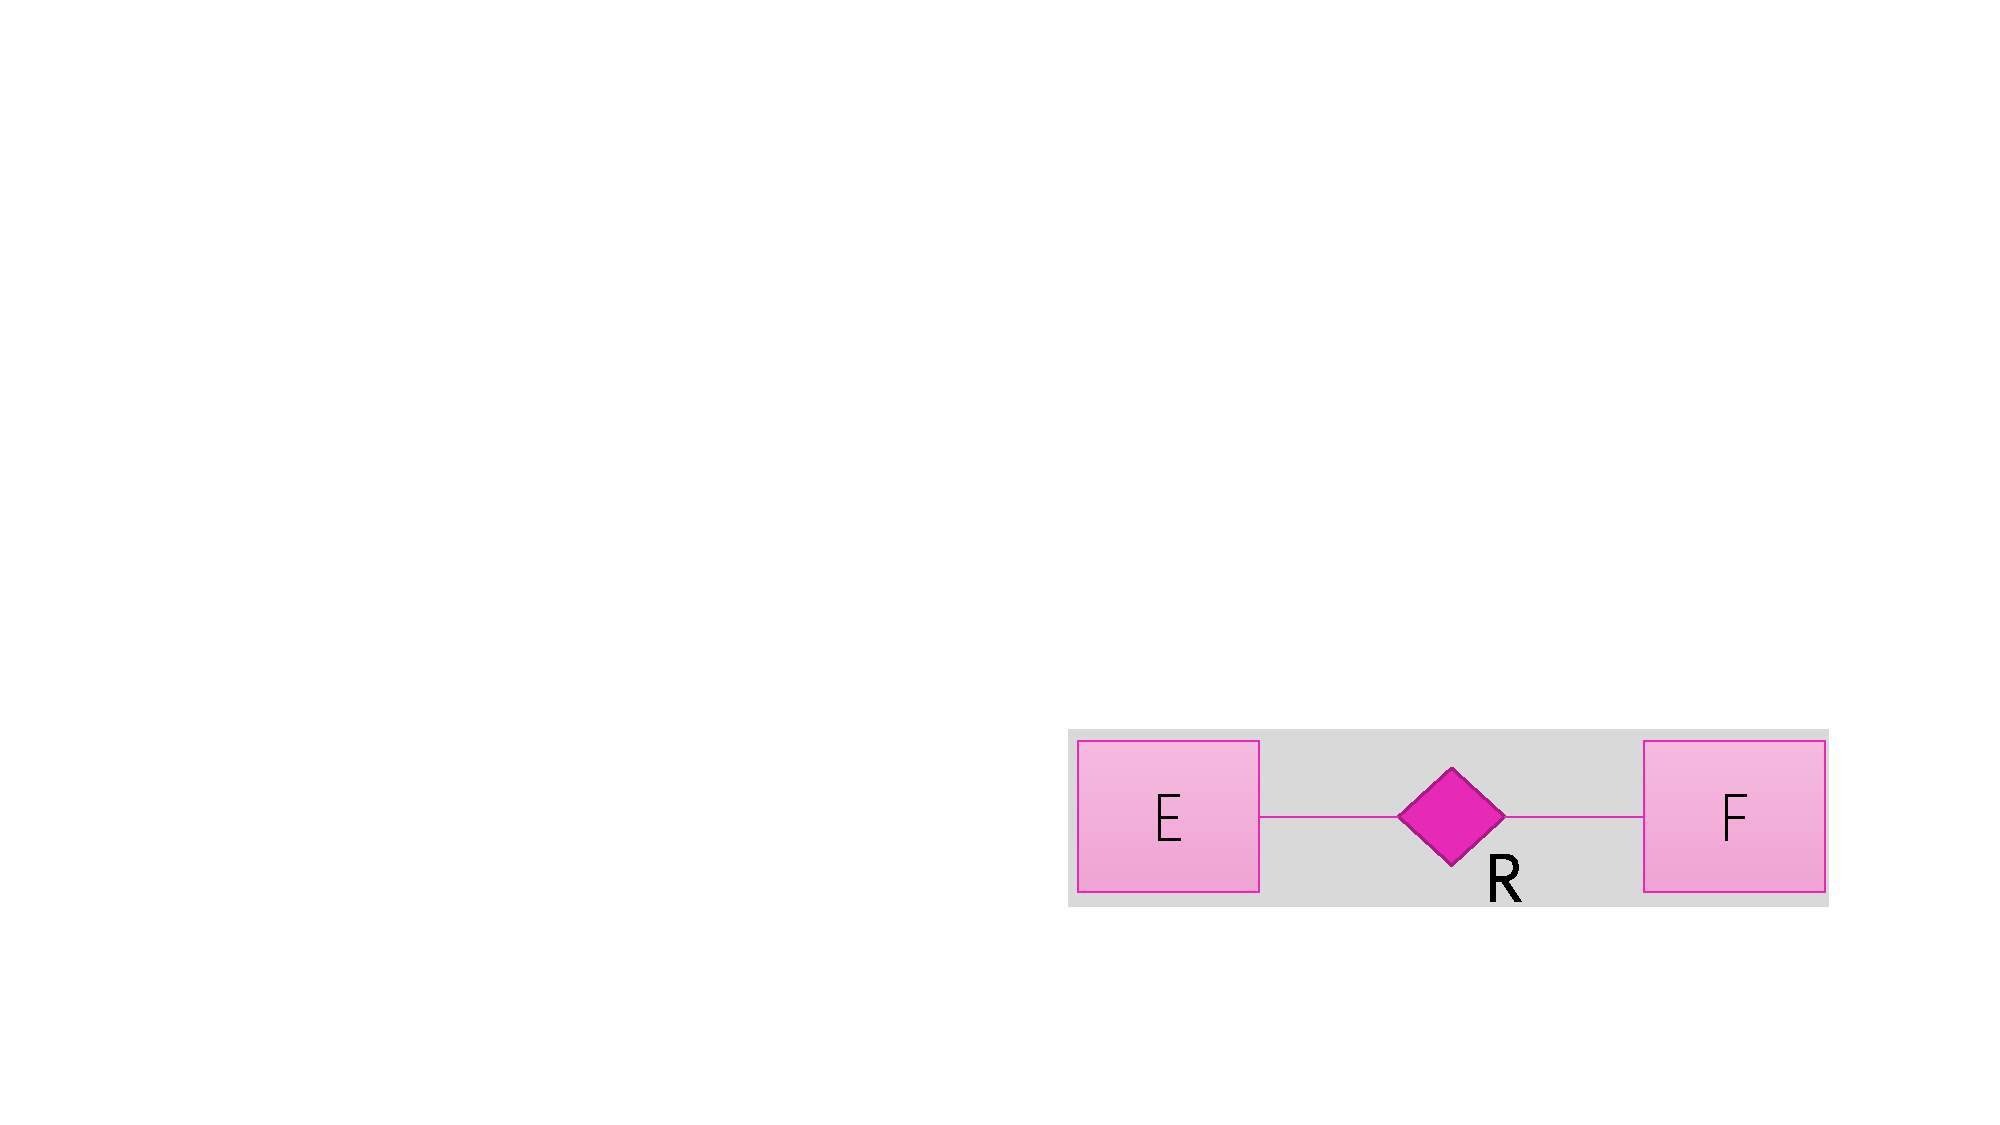
\includegraphics[width=0.6\textwidth]{img/relazione_def.pdf}
		\caption{Sintassi grafica della relazione.}
	\end{figure}

	\noindent
	\textcolor{blue}{\textbf{Istanza (o occorrenza).}} Un'istanza di relazione è un'\textbf{ennupla costituita da istanze di entità, una per ciascuna delle entità coinvolte}.
	
	\noindent
	Data una relazione $R$ tra $n$ entità $E_1, \cdots, E_n$, un’istanza della relazione $R$ è una ennupla di istanze di entità:
	
	\begin{equation*}
		\left(e_1, \cdots, e_n\right) \text{ dove } e_i \in I(E_i), 1\le i \le n
	\end{equation*}

	\noindent
	Infine, esiste una relazione importante. Data una relazione $R$ tra $n$ entità, vale sempre la seguente proprietà sull’insieme delle istanze di $R (I(R))$:
	
	\begin{equation*}
		I(R) \subseteq I(E_1) \times \cdots \times I(E_n)
	\end{equation*}
	
	\newpage
	
	
	
	
	\subsubsection{Attributi}\label{attributi}
	
	\textcolor{Red3}{\textbf{Definizione.}}
	
	\noindent
	\textcolor{Green4}{\textbf{Sintassi grafica.}}
	
%	\begin{figure}[!htp]
%		\centering
%		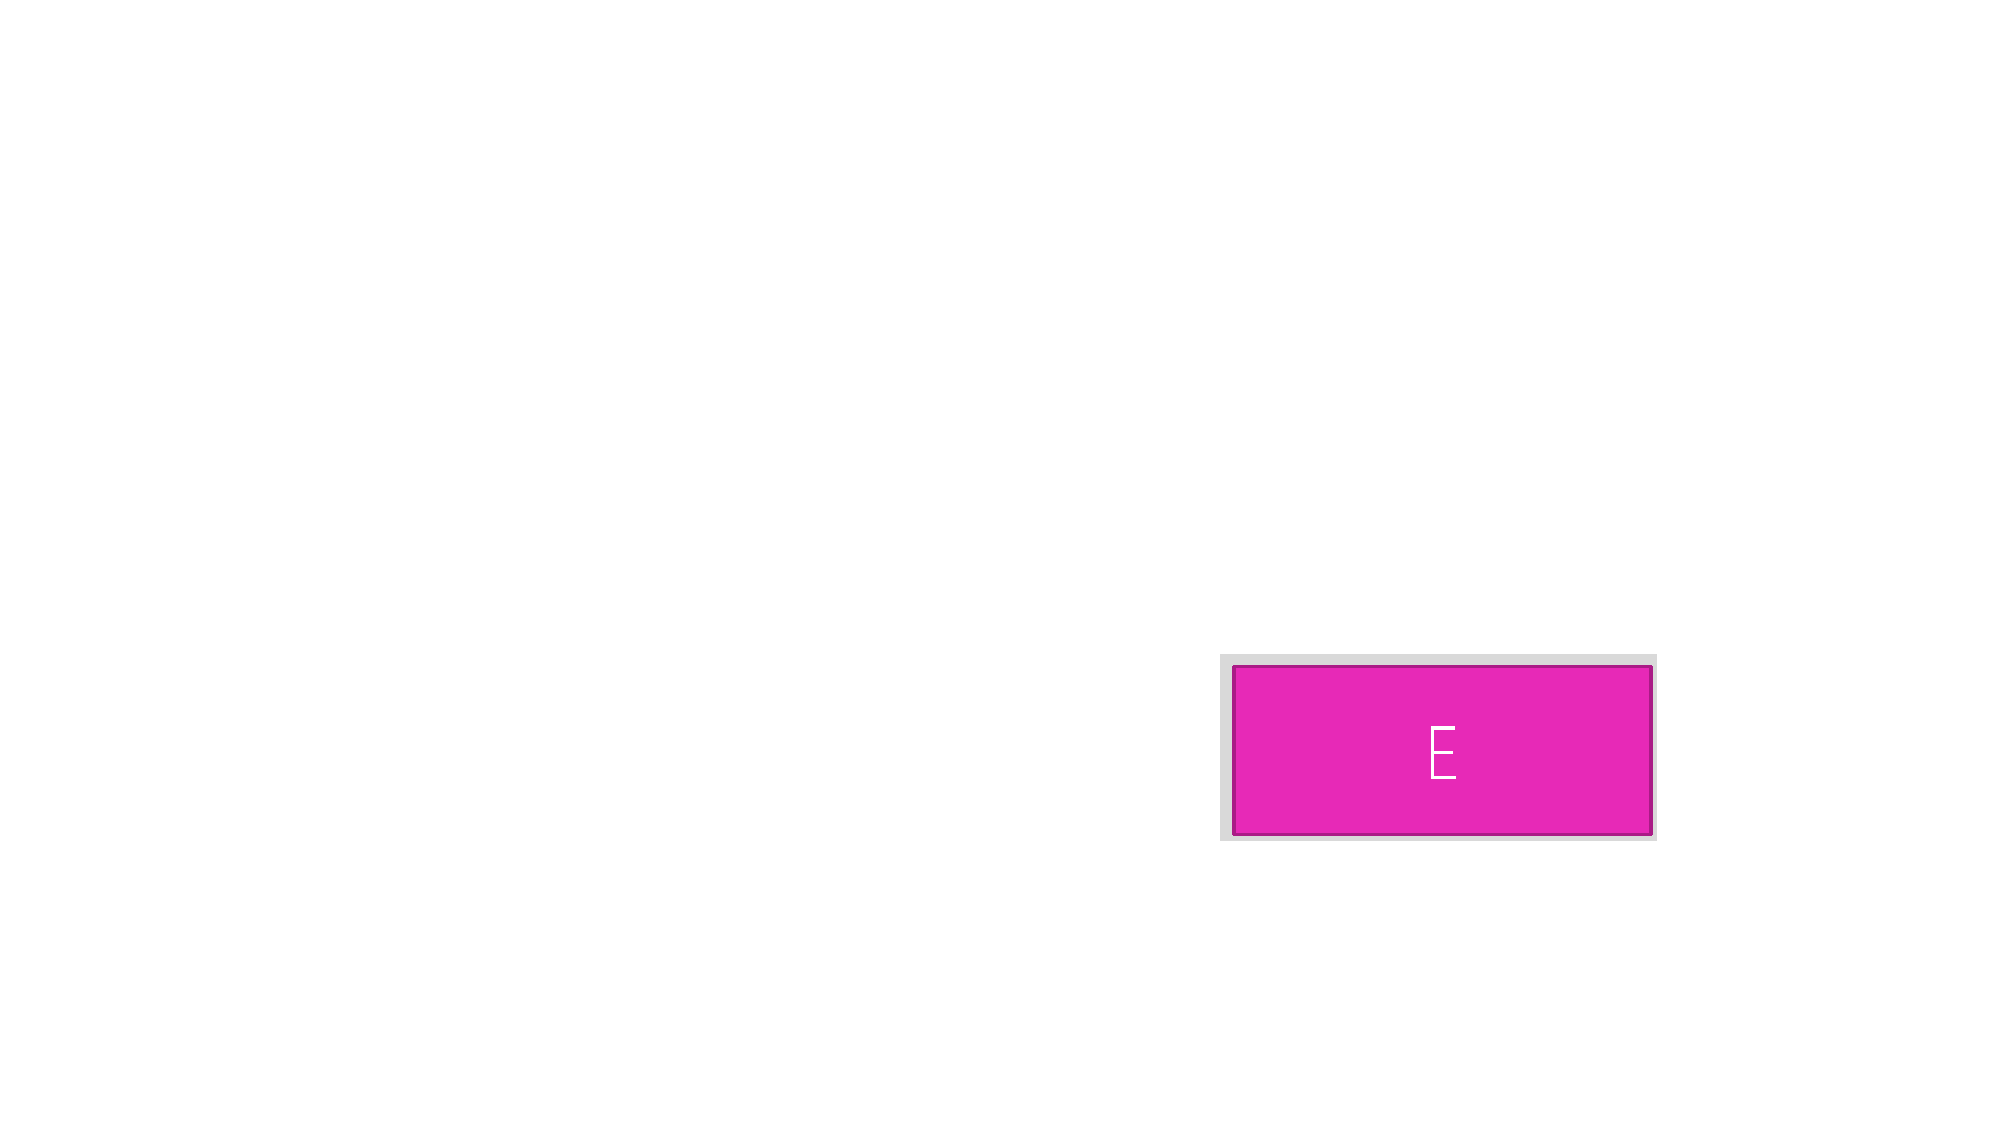
\includegraphics[width=0.5\textwidth]{img/entita_def.pdf}
%		\caption{Sintassi grafica dell'entità.}
%	\end{figure}
	
	\noindent
	\textcolor{blue}{\textbf{Istanza (o occorrenza).}}
\end{document}